\subsubsection{Mint}

Am Host-PC muss bei den IPv4-Einstellungen die Methode "`Automatisch"' eingestellt sein. Wenn es sich um eine neue Verbindung handelt, ist dies bereits voreingestellt, eine Parametrierung kann dann entfallen. Ansonsten muss zur Konfiguration unter Linux (Mint XFCE) zuerst der Dialog "`Netzwerkverbindungen"' ge�ffnet werden.\\ 
Dazu klickt man mit der rechten Maustaste auf das Netzwerksymbol in Infobereich rechts unten. Dann kann die Option "`Netzwerkverbindungen bearbeiten..."' ausgew�hlt werden.

\begin{figure}[ht]
  \centering
  
\includegraphics[scale=1.00]{images/OTG_NetzwerkverbindungenIconMintXFCE.png}	
  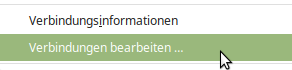
\includegraphics[scale=0.42]{images/OTG_NetzwerkverbindungenOpenMintXFCE.png}	
  %	\caption{}
  \label{OTG_LINUX_NetzwerkverbindungenApp}
\end{figure}


Nun k�nnte die neue "`Kabelnetzwerkverbindung 2"' umbenannt werden, z.~B. in Raspberry Pi Zero. Erkennen kann man das Netzwerk an der Mac-Adresse, die man bei "`g\_ether.host\_addr"' angegeben hat (z.~B. 00:01:02:03:04:05).  


\begin{figure}[ht]
  \centering
	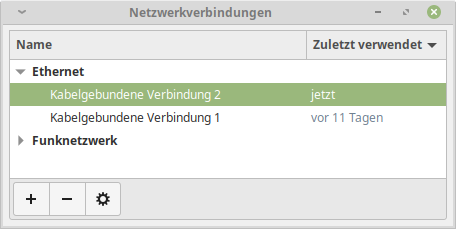
\includegraphics[scale=0.38]{images/OTG_NetzwerkverbindungenMintXFCE.png}
  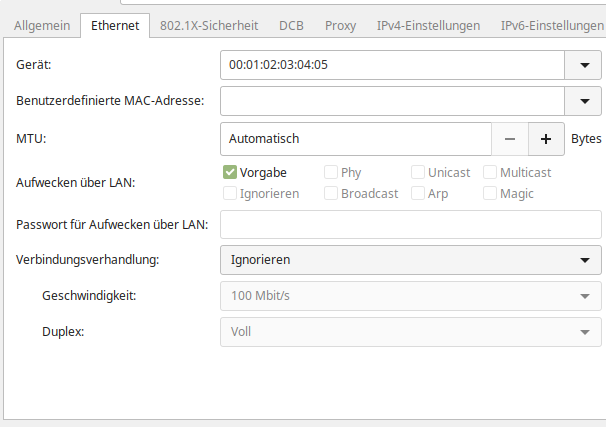
\includegraphics[scale=0.38]{images/OTG_Pi_VerbindungsnameMintXFCE.png}
%	\caption{}
  \label{OTG_LINUX_Netzwerkverbindungen}
\end{figure}


Nun kann bei den IPv4-Einstellungen die Methode "`Automatisch"' eingestellt werden.

\begin{figure}[ht]
  \centering
  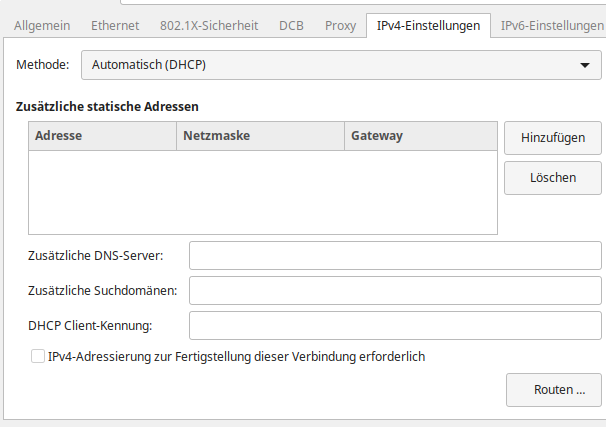
\includegraphics[scale=0.38]{images/OTG_NetzwerkverbindungenAutomatischMintXFCE.png}
	\caption{}
  \label{OTG_LINUX_Netzwerkverbindungen_Auto}
\end{figure}
